\documentclass[a4paper, british]{article}

\usepackage[utf8]{inputenc}
\usepackage[T1]{fontenc}
\usepackage{babel}
% \usepackage[margin=2.5cm,a4paper]{geometry}
% \usepackage[skip=1em]{parskip}
\usepackage{lmodern} 
\usepackage{microtype}
% \usepackage{xcolor}
\usepackage{graphicx}
\graphicspath{ {./figures/} }
% \usepackage{float}
% \usepackage{enumitem}
\usepackage{adjustbox} % rescale - useful for Dia exported TeX
\usepackage{tikz}
% \usepackage{pgfplots}
\usepackage{booktabs} %tables no vertical lines
% \usepackage{array}
% \usepackage{authblk}
% \usepackage{fancyhdr} %headers and footers
% \usepackage{titlesec}
% \usepackage{tcolorbox} % framed text boxes
% \usepackage{mathtools, amssymb, amsthm}
% \usepackage{gensymb}
\usepackage{chemformula} % chemical formulae
\usepackage{chemfig} % molecular figures
\usepackage{siunitx}
\usepackage{csquotes}
\usepackage[titletoc, title]{appendix}
% \usepackage{lettrine} % initials

\usepackage[
pdfauthor={Adam Menne},
pdftitle={Chemistry 264 - Practical 2},
pdfsubject={},
pdfkeywords={}]{hyperref}

\usepackage[noabbrev]{cleveref}

\usepackage[
backend=biber,
style=numeric,
sorting=none,
doi=true,
isbn=false
]{biblatex}
\addbibresource{citations.bib}

\setlength{\parskip}{1em}
\setlength{\parindent}{0em}
\linespread{1.3}

\title{Chemistry 264\\ Practical 2}
\date{Last editted on \today}
\author{Adam Menne\\ Stellenbosch University}

\begin{document}

\maketitle

\begin{abstract}
\noindent
In this practical a chloride solution is standardised by titration with Silver nitrate. From which the composition of the chloride solution was investigated
\end{abstract}

\tableofcontents

\newpage

\section{Introduction}

In this practical we carry out a series of precipitation titrations in order to standardise a chloride solution containing NaCl and KCl. The percent composition of this solution was then found. Potassium chromate was used as an indicator

% \begin{figure}[htb]
%     \centering
%     \chemfig{
%         HO% 3
% -[:330,,2]% 1
%            (
%      =[:270]O% 4
%            )
%   -[:30]% 2
%            (
%       =[:90]O% 6
%            )
% -[:330,,,1]OH% 5
% }
% \end{figure}

\section{Results}

We find that our titrations were relatively consistent, \cref{fig:mean} shows the concentration of \(Cl^-\), calculated over eight titrations. These values have a relative standad deviation of 3.548 as can be seen in \cref{table:data}, which also shows the mean and CI values.

\begin{figure}[h]
    \centering
    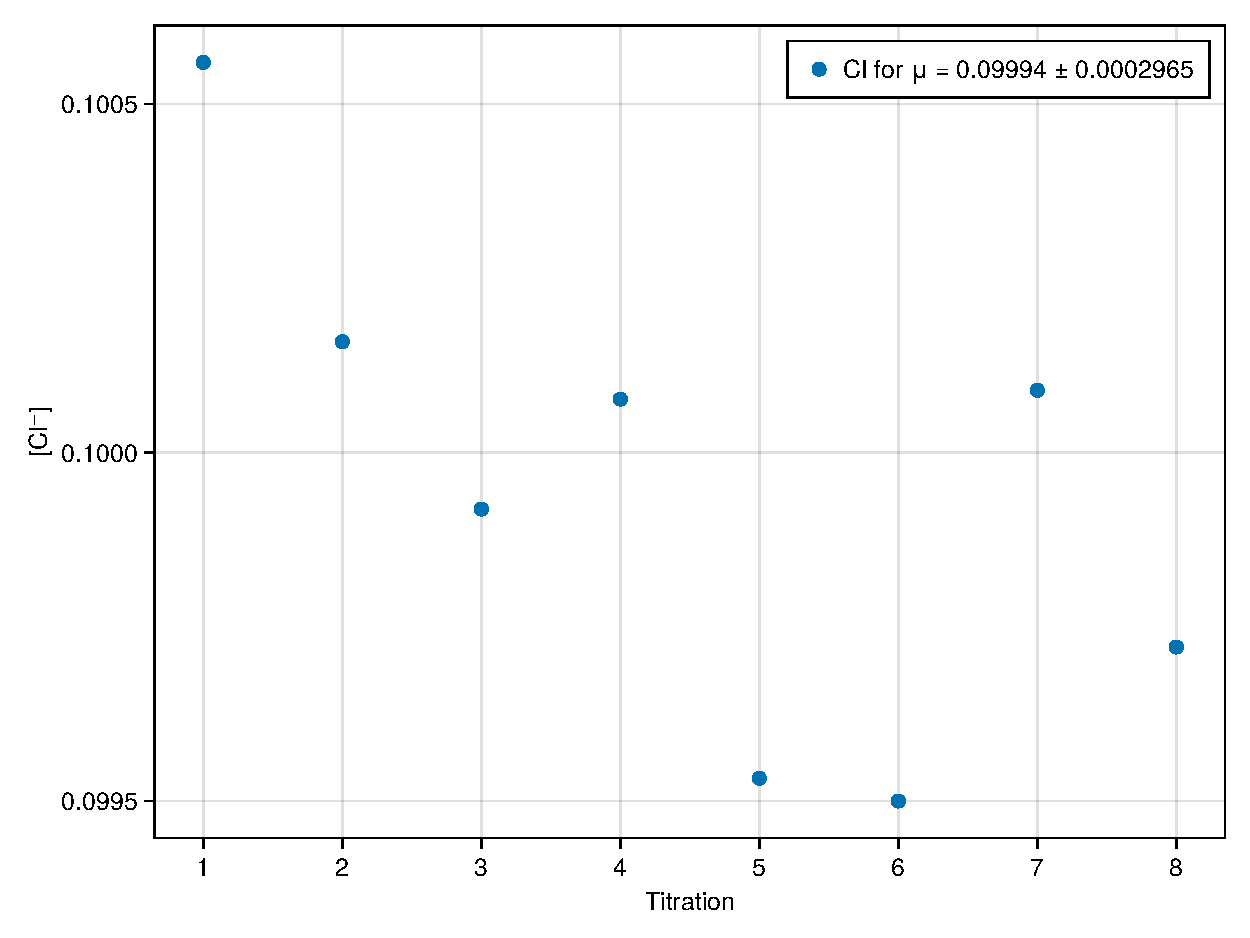
\includegraphics[width=\textwidth]{figures/conc.pdf}
    \caption{Concentration of \(Cl^-\)}
    \label{fig:mean}
\end{figure}

\vspace{25mm}

\begin{table}[h]
    \centering
    \caption{Supplementary Data}
    \begin{tabular}{llc}
        \addlinespace
        \toprule
        Mean & RSD & CI\\ 
        \midrule
        0.09994 & 3.458 & 0.09965 - 0.1002\\
        \bottomrule
        \end{tabular}
        \label{table:data}   
\end{table}

A static export of the notebook containing all analysis and figures is availible at \url{https://adammenne.github.io/chemistry_264/practical_2/plots.html}. With full source code availble at \url{https://github.com/AdamMenne/chemistry_264/tree/master/practical_2}

\section{Discussion}

From the titrations that were carried out, the metrics of relative standard deviation and confidence intervals for the mean, show that the titrations were consistent and precise. 

However improvements are possible by increasing the number of titrations carried out, and utilising a more accurate and precise method of identifying when the equivalence point has been reached.

\newpage

\begin{appendices}
    \section{Flow diagram}

    \begin{enumerate}
        \item Fill one burette with chloride solution, fill another with Silver nitrate solution.
        \item Add 1ml Potassium chromate to an Erlenmeyer flask. Add 10ml of the chloride solution.
        \item Titrate, swirling constantly.
        \item Tabulate titration values
    \end{enumerate}

    \subsubsection*{Silver Nitrate}
    \begin{itemize}
        \item Oxidising
        \item Corrosive
        \item Toxic
        \item Environmental Hazard
        \item[-] avoid contact with skin and eyes
        \item[-] may intensify fires
        \item[-] wash immediately if contact occurs
      \end{itemize}

      \subsubsection*{Potassium Chromate}
      \begin{itemize}
          \item Harmful
          \item Health Hazard
          \item Environmental Hazard
          \item[-] avoid contact with skin and eyes, do not inhale
          \item[-] wash immediately if contact occurs
        \end{itemize}

    \newpage
    
\end{appendices}

\end{document}